\documentclass[10pt,twocolumn]{article}

% ── Packages ──
\usepackage[utf8]{inputenc}
\usepackage[T1]{fontenc}
\usepackage{times}            % Times font (arXiv standard)
\usepackage{microtype}
\usepackage{graphicx}
\usepackage{booktabs}
\usepackage{amsmath,amssymb}
\usepackage{xcolor}
\usepackage{hyperref}
\usepackage{caption}
\usepackage{subcaption}
\usepackage{enumitem}
\usepackage{multirow}
\usepackage{array}
\usepackage[margin=1in]{geometry}
\usepackage{fancyhdr}
\usepackage{natbib}
\usepackage{float}
\usepackage{textcomp}
\usepackage{newunicodechar}
\DeclareRobustCommand{\promptchar}{{\fontfamily{cmr}\selectfont\guilsinglright}}

% ── Colors ──
\definecolor{linkblue}{HTML}{2980b9}
\definecolor{darkaccent}{HTML}{2c3e50}
\definecolor{lightgray}{HTML}{f5f5f5}
\definecolor{correctgreen}{HTML}{27ae60}
\definecolor{wrongred}{HTML}{e74c3c}

\hypersetup{
  colorlinks=true,
  linkcolor=linkblue,
  citecolor=linkblue,
  urlcolor=linkblue,
}

% ── Caption style ──
\captionsetup{font=small,labelfont=bf}

% ── Reduce spacing ──
\setlength{\columnsep}{0.25in}
\setlist{nosep,leftmargin=*}

% ── Header ──
\pagestyle{fancy}
\fancyhf{}
\fancyhead[L]{\small\textit{Does Claude Know How Its Harness Looks Like?}}
\fancyhead[R]{\small\thepage}
\renewcommand{\headrulewidth}{0.4pt}

% ── Graphics path ──
\graphicspath{{../../figures/v2/}}

% ══════════════════════════════════════════════════════════════
\begin{document}

% ── Title (single column) ──
\twocolumn[
\begin{@twocolumnfalse}
\begin{center}
\vspace*{0.3cm}
{\LARGE\bfseries Does Claude Know How Its Harness Looks Like?\\[6pt]}
{\large A Systematic Evaluation of LLM Self-Knowledge\\
About Its Deployment Interface\\[12pt]}
{\normalsize
Hyogon Ryu\\
\textit{KRAFTON Inc.}\\[4pt]
{\small March 2026}\\[8pt]
}
\end{center}

% ── Abstract ──
\begin{center}
\begin{minipage}{0.92\textwidth}
\textbf{Abstract.}
We investigate whether large language models possess accurate knowledge about the visual appearance of their deployment interface.
Specifically, we test Claude (Sonnet 4.6) on its knowledge of the Claude Code CLI---the terminal-based harness through which it is deployed.
We design 55 prompts spanning 10 mutually exclusive domains and 5 cognitive demand types (free recall, forced choice, true/false, spatial reasoning, exact detail).
Our structured evaluation reveals \textbf{82.1\% objective accuracy} on 28 forced-choice and true/false items, with an average confidence of 0.588 and calibration error of 0.430.
The model achieves perfect accuracy on negative knowledge probes (correctly identifying non-existent features) but struggles with navigation shortcuts (33\%) and recently-added features like Vim mode and output styles.
These results suggest LLMs have structured but incomplete meta-knowledge of their deployment environment, with systematic blind spots in visual-only and feature-specific details.

\vspace{4pt}
\noindent\textbf{Keywords:} LLM self-knowledge, meta-cognition, hallucination, Claude Code, deployment interface, confidence calibration
\end{minipage}
\end{center}
\vspace{0.4cm}
\end{@twocolumnfalse}
]

% ══════════════════════════════════════════════════════════════
\section{Introduction}

Large language models (LLMs) are increasingly deployed through specialized interfaces---terminal CLIs, web applications, IDE integrations---that mediate the user experience.
Yet we know little about whether these models possess accurate knowledge of the interfaces that host them.
This question has practical implications: if an LLM can describe its own interface, it may better assist users with interface-related tasks; if it cannot, it risks confidently hallucinating visual details that mislead users.

We address the research question: \textbf{Does Claude know how its harness (Claude Code CLI) looks like?}
We systematically evaluate Claude's knowledge across 10 interface domains using 55 carefully designed prompts spanning 5 cognitive demand types.
This extends prior work on LLM self-knowledge by focusing specifically on \textit{visual and spatial} knowledge of the deployment environment.

Our key contributions are:
\begin{enumerate}
  \item A structured evaluation framework with MECE domain taxonomy and mixed prompt types including negative knowledge controls;
  \item A ground truth database of 74 verified facts about Claude Code built from screenshots, documentation, and empirical session observation;
  \item Empirical results showing 82.1\% objective accuracy with systematic blind spots in navigation and recently-added features;
  \item Analysis of confidence calibration revealing appropriate uncertainty in knowledge gaps.
\end{enumerate}

% ══════════════════════════════════════════════════════════════
\section{Related Work}

\paragraph{LLM Self-Knowledge.}
Prior studies have examined whether LLMs know their own capabilities, training data composition, and knowledge boundaries~\citep{kadavath2022language,yin2023large}.
Our work extends this to \textit{deployment-context} knowledge---what the model knows about the interface wrapping it.

\paragraph{Hallucination in Visual Descriptions.}
LLMs frequently hallucinate visual details when asked to describe images or interfaces they have not seen~\citep{ji2023survey}.
Our prompts are designed to detect such hallucinations through forced-choice items and negative probes.

\paragraph{Confidence Calibration.}
Well-calibrated models express appropriate uncertainty when they lack knowledge~\citep{guo2017calibration}.
We analyze per-item confidence alongside accuracy to assess calibration quality.

% ══════════════════════════════════════════════════════════════
\section{Methodology}

\subsection{Target Interface}
Claude Code v2.1.66 is Anthropic's official terminal-based CLI for Claude.
It features a rich text interface with Unicode box-drawing, two-column startup layout, inline permission dialogs, interactive diff views, 6 color themes, and extensive keyboard shortcuts.
It is built with Ink (React for CLI) and runs on macOS, Linux, and Windows.

\subsection{Domain Taxonomy}
We organize interface knowledge into 10 mutually exclusive, collectively exhaustive (MECE) domains, shown in Table~\ref{tab:domains}.
Domain D10 (Negative Space) serves as a control condition, testing features that do \textit{not} exist in Claude Code.

\begin{table}[t]
\centering
\caption{Ten evaluation domains with prompt counts.}
\label{tab:domains}
\small
\begin{tabular}{@{}clc@{}}
\toprule
\textbf{ID} & \textbf{Domain} & \textbf{\#P} \\
\midrule
D1  & Startup / Welcome Screen & 7 \\
D2  & Input Area \& Prompt & 6 \\
D3  & Output \& Response Display & 6 \\
D4  & Permission / Approval Dialogs & 6 \\
D5  & Status Line \& Footer & 5 \\
D6  & Navigation \& Commands & 6 \\
D7  & Theming \& Colors & 5 \\
D8  & Diff \& File Editing & 5 \\
D9  & Error \& Edge States & 4 \\
D10 & Negative Space (Control) & 5 \\
\midrule
    & \textbf{Total} & \textbf{55} \\
\bottomrule
\end{tabular}
\end{table}

\subsection{Cognitive Type Taxonomy}
Each prompt employs one of five cognitive demand types:
\textbf{T1}~Free Recall (open-ended ``describe X'');
\textbf{T2}~Forced Choice (4-option multiple choice, 25\% chance);
\textbf{T3}~True/False (binary, 50\% chance);
\textbf{T4}~Spatial Reasoning (``what is above/below X'');
\textbf{T5}~Exact Detail (``what exact character is used for Y'').
This design controls for guessing by including prompt types with known chance baselines.

\subsection{Prompt Design}
We designed 55 prompts covering all cells of the $10 \times 5$ domain-type matrix.
Prompts include:
\begin{itemize}
  \item \textbf{Hallucination probes}: e.g., P03 tests the known ``CLAUDE CODE'' ASCII banner fabrication;
  \item \textbf{Negative probes}: D10 tests features that don't exist (sidebar, avatars, inline images);
  \item \textbf{Detail probes}: e.g., P09 tests the exact prompt character (\texttt{>} vs U+276F).
\end{itemize}
All prompts enforce structured JSON output with per-claim confidence scores.

\subsection{Ground Truth}
We compile a ground truth database of 74 verified facts from three sources:
\begin{enumerate}
  \item \textbf{Screenshot analysis} of an actual Claude Code v2.1.66 startup screen, confirming the two-column layout, U+276F prompt character, and small abstract logo;
  \item \textbf{Official documentation} at \texttt{code.claude.com} covering 25 UI categories;
  \item \textbf{Empirical session observation} including system prompt inspection and CLI help output.
\end{enumerate}
Each fact is tagged with source, domain, and confidence level (definitive / documented / empirical).

\subsection{Evaluation Protocol}
We evaluate Claude Sonnet 4.6 using subagent instances with explicit instructions to answer from training knowledge only (no tool use).
Objective prompts (T2, T3) are scored by direct answer comparison.
Free-recall prompts (T1, T4, T5) are scored using keyword-based claim matching against the GT database.
Per-claim confidence enables calibration analysis.

% ══════════════════════════════════════════════════════════════
\section{Results}

\subsection{Overall Performance}

Claude achieves \textbf{82.1\% objective accuracy} on 28 forced-choice and true/false items, substantially above both T/F chance (50\%) and 4-choice chance (25\%).
The model produced 106 atomic claims in free-recall responses, with 86 verified correct and 20 unverifiable.
Average stated confidence is 0.588, with calibration error of 0.430.

\begin{table}[t]
\centering
\caption{Results by domain. Obj.\ Acc.\ = accuracy on objective items (T2+T3). Claims = total atomic claims from free-recall. Conf.\ = average stated confidence.}
\label{tab:results}
\small
\begin{tabular}{@{}llcrc@{}}
\toprule
\textbf{Dom.} & \textbf{Description} & \textbf{Obj.Acc.} & \textbf{Cl.} & \textbf{Conf.} \\
\midrule
D1  & Startup Screen        & 67\%  & 16 & .52 \\
D2  & Input Area            & 67\%  & 14 & .58 \\
D3  & Output Display        & 67\%  & 12 & .77 \\
D4  & Permission Dialogs    & \textcolor{correctgreen}{100\%} & 13 & .67 \\
D5  & Status Line           & \textcolor{correctgreen}{100\%} & 10 & .43 \\
D6  & Navigation            & \textcolor{wrongred}{33\%}  & 15 & .37 \\
D7  & Theming               & \textcolor{correctgreen}{100\%} &  9 & .20 \\
D8  & Diff / Editing        & \textcolor{correctgreen}{100\%} &  9 & .50 \\
D9  & Error States          & \textcolor{correctgreen}{100\%} &  8 & .40 \\
D10 & Negative (Ctrl.)      & \textcolor{correctgreen}{100\%} &  0 & .94 \\
\midrule
    & \textbf{Overall}      & \textbf{82.1\%} & \textbf{106} & \textbf{.59} \\
\bottomrule
\end{tabular}
\end{table}

\subsection{Domain Analysis}

\paragraph{Strongest domains.}
D10 (Negative Space), D4 (Permission), D5 (Status), D7 (Theming), D8 (Diff), and D9 (Error) all achieve 100\% objective accuracy.
The model excels at both negative knowledge---knowing what \textit{doesn't} exist---and functional knowledge about permission systems and diff views.

\paragraph{Weakest domain.}
D6 (Navigation) scores only 33\%, \textit{below} T/F chance level.
The model incorrectly denied the existence of Vim mode (\texttt{/vim} command), chose \texttt{Ctrl+E} instead of \texttt{Ctrl+G} for the external editor shortcut, and guessed \texttt{Ctrl+R} for permission mode cycling (correct: \texttt{Shift+Tab}).

\paragraph{Moderate domains.}
D1 (Startup, 67\%), D2 (Input, 67\%), D3 (Output, 67\%).
The model correctly identified the two-column startup layout and the U+276F prompt character but missed the personalized greeting, all multiline input methods, and the existence of three output styles.

\subsection{Error Analysis}

Table~\ref{tab:errors} details all 5 wrong answers.
A clear pattern emerges: the model lacks knowledge of \textbf{recently-added features} (Vim mode, output styles, personalized greeting) and \textbf{specific keyboard shortcuts} (\texttt{Ctrl+G} vs \texttt{Ctrl+E}).
Notably, wrong answers have lower average confidence (0.55) than correct answers (0.60), suggesting partial calibration.

\begin{table}[t]
\centering
\caption{All 5 wrong answers with confidence and explanation.}
\label{tab:errors}
\small
\begin{tabular}{@{}ccccp{2.8cm}@{}}
\toprule
\textbf{ID} & \textbf{Ans.} & \textbf{GT} & \textbf{Conf.} & \textbf{Explanation} \\
\midrule
P06 & F & T & .55 & Personalized greeting (``Welcome back [Name]!'') exists \\
P13 & A & D & .55 & All 3 multiline methods work (Shift+Enter, \textbackslash+Enter, Ctrl+J) \\
P19 & F & T & .80 & 3 output styles exist (Default, Explanatory, Learning) \\
P33 & F & T & .45 & Built-in Vim mode (\texttt{/vim}) exists \\
P36 & A & B & .40 & External editor is Ctrl+G, not Ctrl+E \\
\bottomrule
\end{tabular}
\end{table}

\subsection{Confidence Calibration}

The model shows meaningful but imperfect calibration (Figure~\ref{fig:calibration}).
Average confidence for correct answers (0.60) exceeds that for incorrect ones (0.55), demonstrating metacognitive awareness.
However, calibration error of 0.430 indicates systematic overconfidence on wrong answers (e.g., P19 at 0.80 confidence) and underconfidence on correct ones.
D10 shows best calibration (0.94 confidence, 100\% accuracy); D7 shows poorest (0.20 confidence, 100\% accuracy).

\subsection{Cognitive Type Analysis}

Forced-choice accuracy (84.6\%, $n{=}13$) slightly exceeds true/false accuracy (80.0\%, $n{=}15$), both substantially above chance baselines (25\% and 50\% respectively).
This confirms the model possesses genuine knowledge rather than randomly guessing.
Free-recall prompts (T1) yield 51 claims from 9 prompts---the richest data but hardest to score.

% ══════════════════════════════════════════════════════════════
\section{Discussion}

\subsection{Knowledge Hierarchy}
Our results reveal a clear knowledge hierarchy:
(1)~\textit{Negative knowledge}---the model accurately knows what its interface is NOT (no sidebar, no avatars, no inline images);
(2)~\textit{Structural knowledge}---general architecture (terminal-based, inline dialogs, diff coloring) is well-understood;
(3)~\textit{Specific features}---recently-added or lesser-known features (Vim mode, output styles, personalized greeting) form blind spots.
This hierarchy likely reflects training data coverage: older, well-documented features are better represented.

\subsection{Calibration Quality}
The model demonstrates appropriate epistemic humility in uncertain domains (D7 Theming: 0.20 confidence, D6 Navigation: 0.37) while showing high confidence in well-known areas (D10: 0.94, D3: 0.77).
The P19 failure (0.80 confidence, wrong) reveals that calibration can break down when the model confuses absence of knowledge with confident disbelief.

\subsection{Implications}
\textbf{For deployment:} Models may confidently describe their interface incorrectly, particularly for features added after the training cutoff.
\textbf{For trust:} The 82\% accuracy means roughly 1 in 5 interface-related claims may be wrong.
\textbf{For development:} Including deployment interface documentation in training data could improve self-knowledge.

% ══════════════════════════════════════════════════════════════
\section{Limitations}

\textbf{Single trial.} Each prompt was evaluated once ($N{=}1$). Repeated trials would enable consistency analysis.
\textbf{Heuristic scoring.} Free-recall claims were scored using keyword matching rather than LLM-based judgment.
\textbf{Context contamination.} Subagents inherit the Claude Code system prompt, which contains tool and platform information, potentially inflating accuracy.
\textbf{Single model.} Only Sonnet 4.6 was tested; Opus and Haiku may differ.
\textbf{Version specificity.} Results apply to Claude Code v2.1.66; newer versions may differ.

% ══════════════════════════════════════════════════════════════
\section{Conclusion}

Claude demonstrates structured but incomplete knowledge of the Claude Code CLI, achieving 82.1\% accuracy on objective questions.
The model excels at negative knowledge (100\%) and structural understanding but has systematic blind spots in navigation shortcuts and recently-added features.
Confidence calibration shows meaningful but imperfect metacognitive awareness.
Future work should extend this evaluation to multiple models, harness types (web UI, IDE plugins), and include repeated trials for statistical robustness.

\vspace{6pt}
\noindent\textbf{Code and data:} \url{https://github.com/ugonfor/claude-code-meta-recognition}

% ══════════════════════════════════════════════════════════════
% Figures
% ══════════════════════════════════════════════════════════════

\begin{figure*}[t]
  \centering
  \begin{subfigure}[t]{0.48\textwidth}
    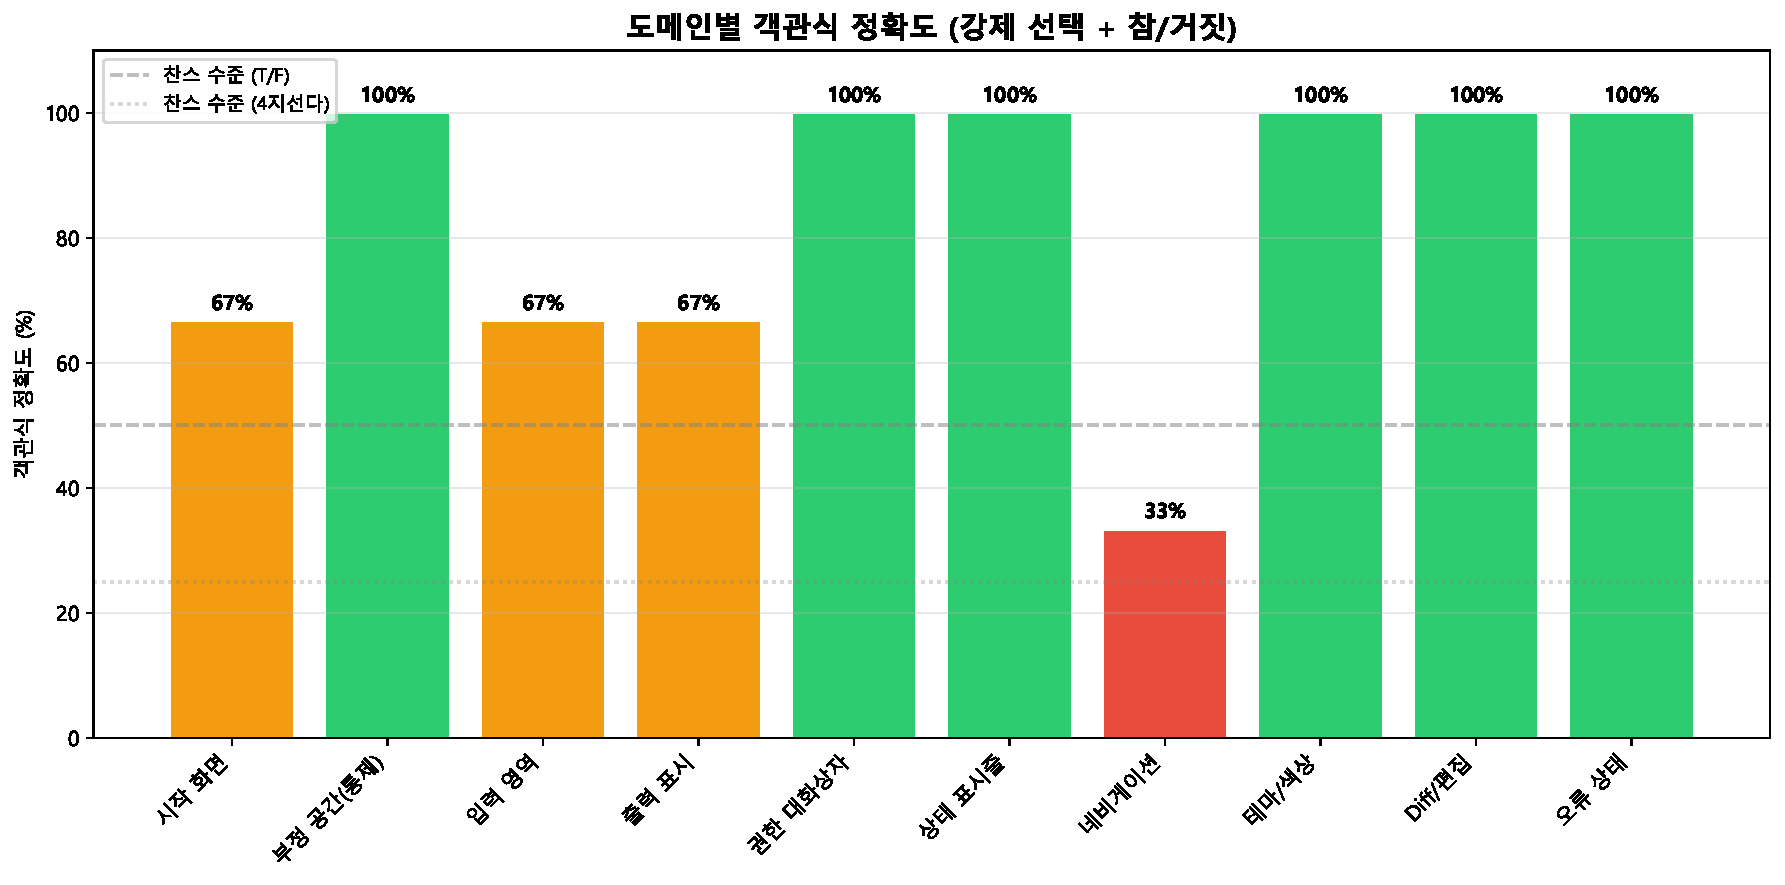
\includegraphics[width=\textwidth]{fig1_domain_accuracy.pdf}
    \caption{Objective accuracy by domain.}
    \label{fig:domain_acc}
  \end{subfigure}
  \hfill
  \begin{subfigure}[t]{0.48\textwidth}
    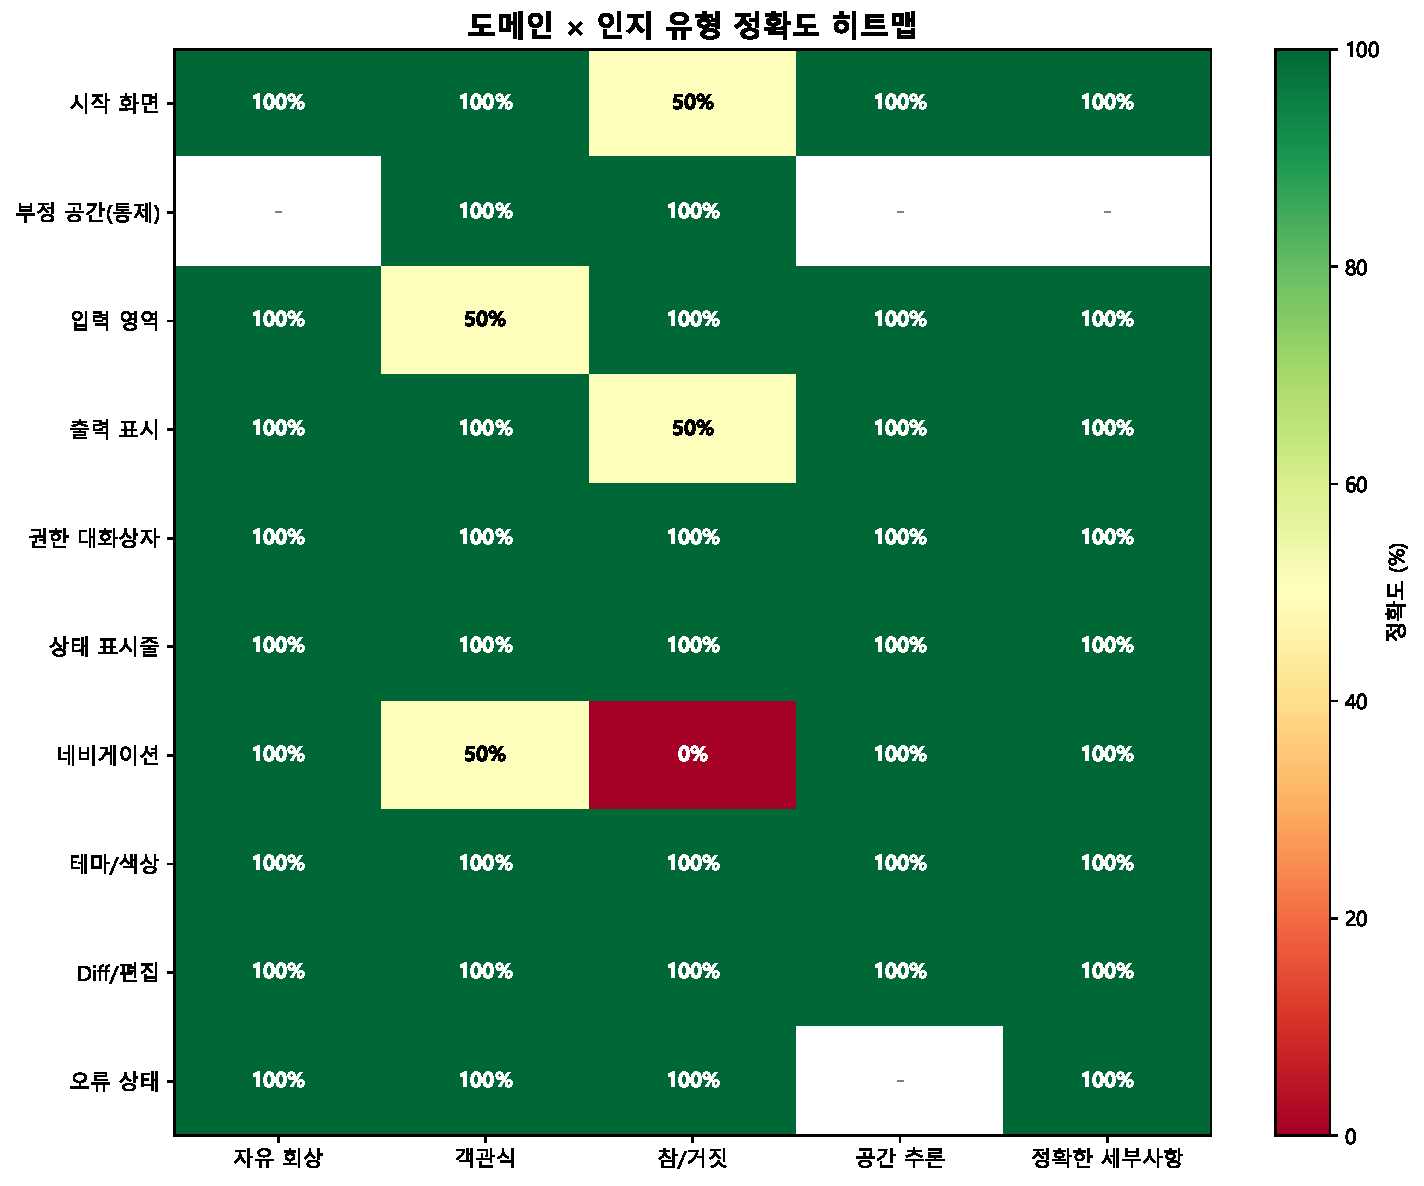
\includegraphics[width=\textwidth]{fig2_heatmap.pdf}
    \caption{Domain $\times$ cognitive type accuracy heatmap.}
    \label{fig:heatmap}
  \end{subfigure}
  \\[8pt]
  \begin{subfigure}[t]{0.48\textwidth}
    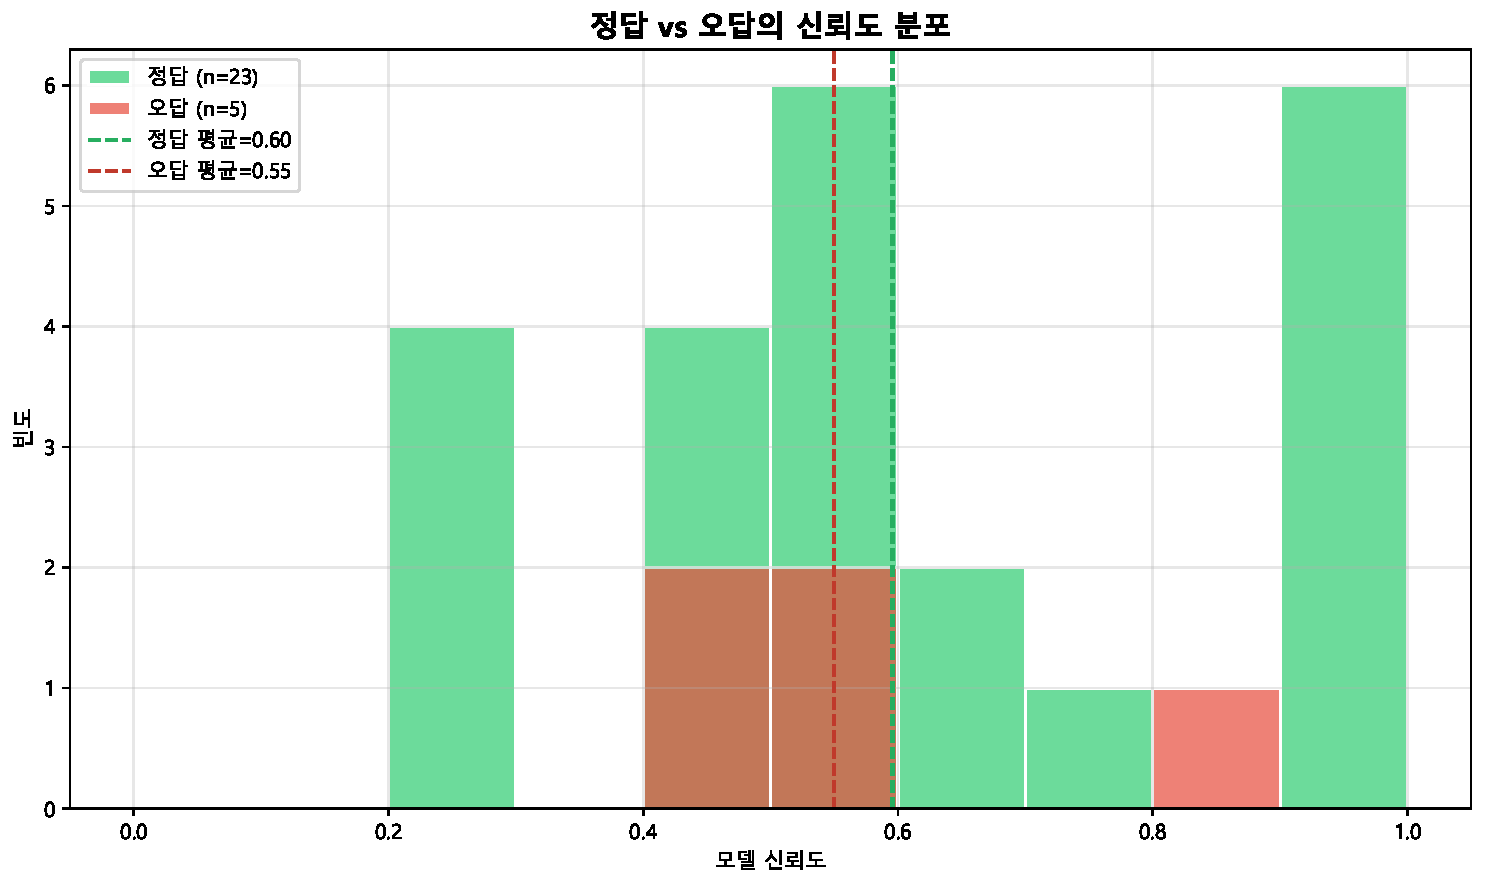
\includegraphics[width=\textwidth]{fig5_confidence_dist.pdf}
    \caption{Confidence distribution: correct vs.\ incorrect answers.}
    \label{fig:conf_dist}
  \end{subfigure}
  \hfill
  \begin{subfigure}[t]{0.48\textwidth}
    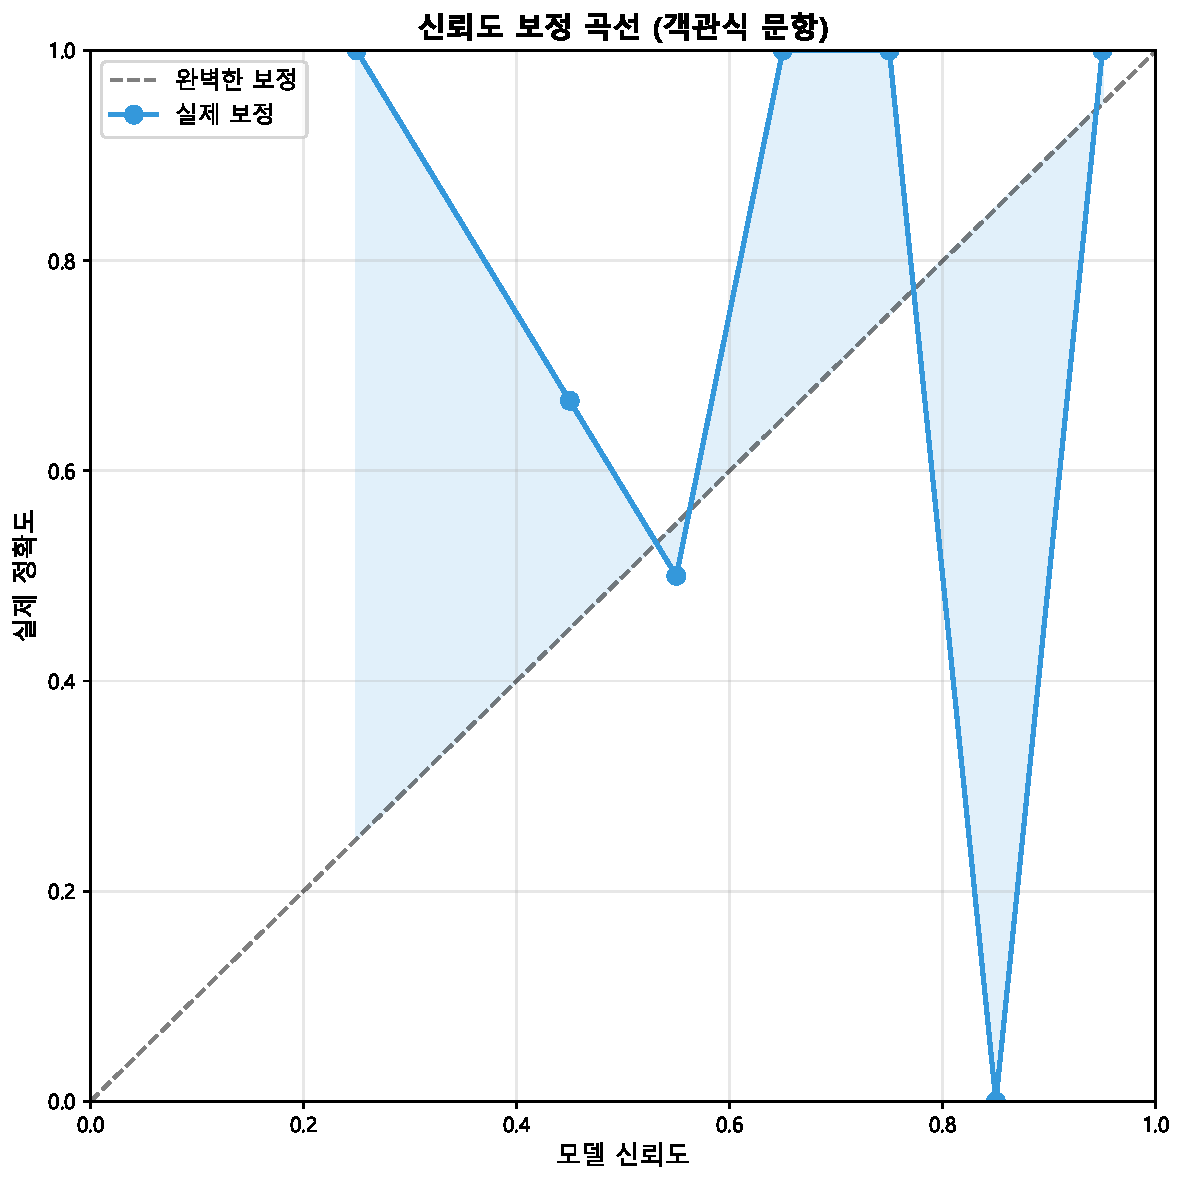
\includegraphics[width=\textwidth]{fig3_calibration.pdf}
    \caption{Confidence calibration curve.}
    \label{fig:calibration}
  \end{subfigure}
  \caption{Main experimental results. (a)~Six domains achieve 100\% while Navigation (D6) drops to 33\%. (b)~The heatmap reveals Navigation$\times$T/F as the weakest cell. (c)~Correct answers cluster at higher confidence than incorrect ones. (d)~The calibration curve shows under-confidence on easy items and over-confidence on hard ones.}
  \label{fig:main_results}
\end{figure*}

\begin{figure}[t]
  \centering
  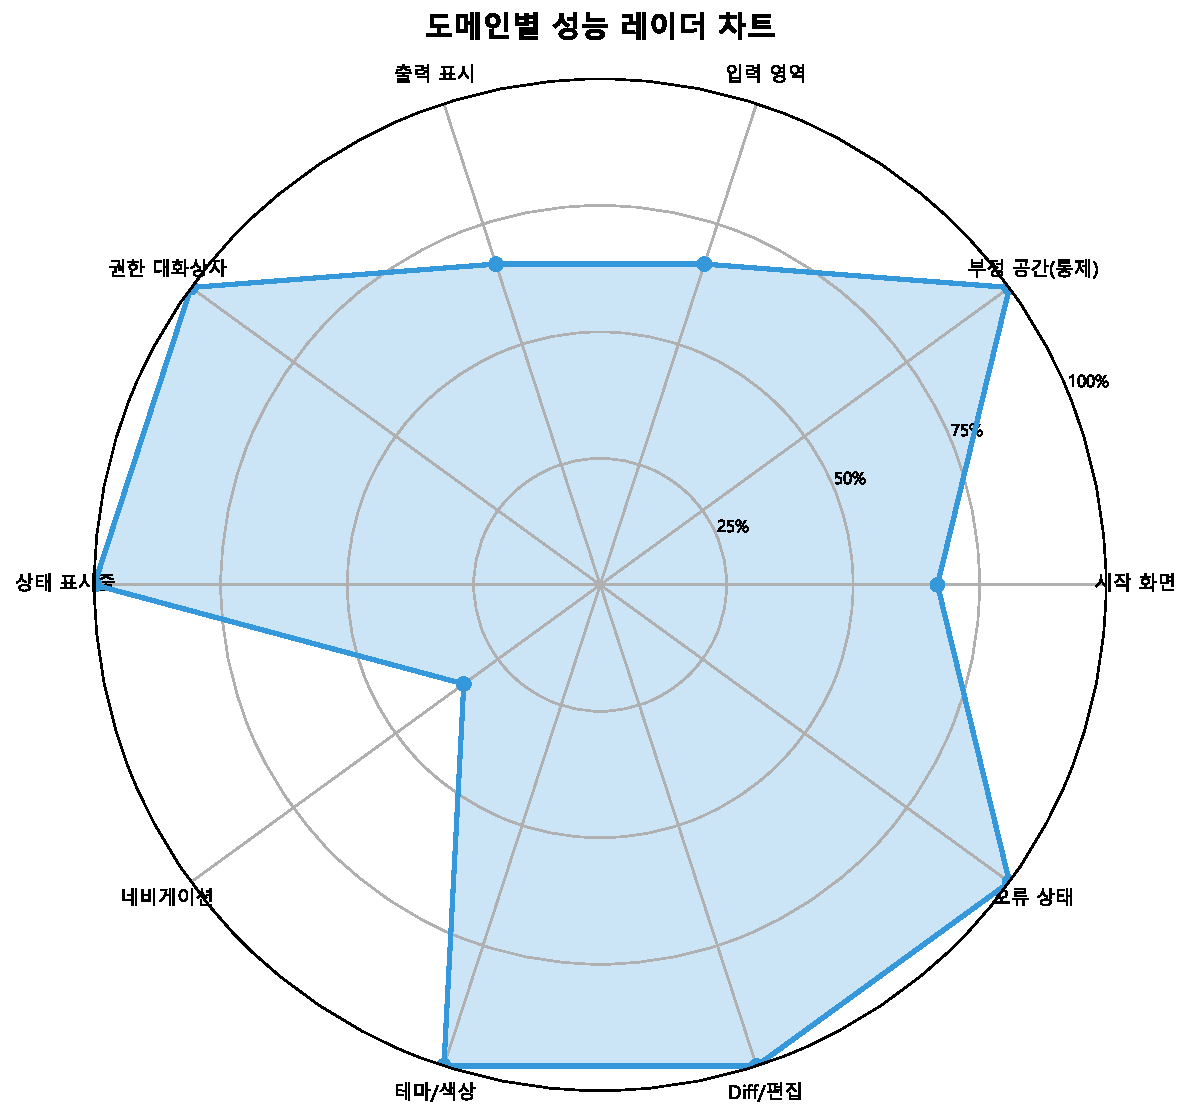
\includegraphics[width=\columnwidth]{fig8_radar.pdf}
  \caption{Radar chart of domain-level performance.}
  \label{fig:radar}
\end{figure}

\begin{figure}[t]
  \centering
  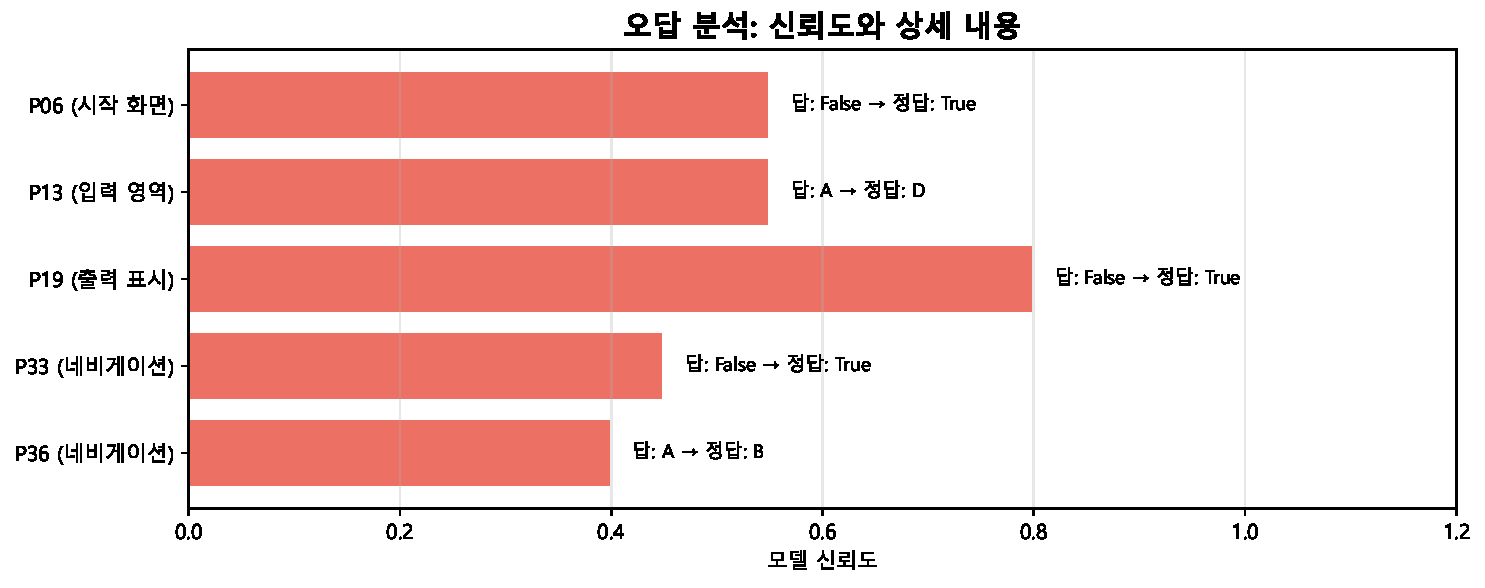
\includegraphics[width=\columnwidth]{fig7_wrong_answers.pdf}
  \caption{Wrong answers with stated confidence levels.}
  \label{fig:wrong}
\end{figure}

% ══════════════════════════════════════════════════════════════
% References
% ══════════════════════════════════════════════════════════════

\bibliographystyle{plainnat}
\begin{thebibliography}{9}

\bibitem[Kadavath et~al.(2022)]{kadavath2022language}
S.~Kadavath, T.~Conerly, A.~Askell, et~al.
\newblock Language models (mostly) know what they know.
\newblock \textit{arXiv preprint arXiv:2207.05221}, 2022.

\bibitem[Yin et~al.(2023)]{yin2023large}
Z.~Yin, Q.~Sun, Q.~Guo, J.~Wu, X.~Qiu, and X.~Huang.
\newblock Do large language models know what they don't know?
\newblock In \textit{Findings of ACL}, 2023.

\bibitem[Ji et~al.(2023)]{ji2023survey}
Z.~Ji, N.~Lee, R.~Frieske, T.~Yu, et~al.
\newblock Survey of hallucination in natural language generation.
\newblock \textit{ACM Computing Surveys}, 55(12):1--38, 2023.

\bibitem[Guo et~al.(2017)]{guo2017calibration}
C.~Guo, G.~Pleiss, Y.~Sun, and K.~Q. Weinberger.
\newblock On calibration of modern neural networks.
\newblock In \textit{ICML}, 2017.

\end{thebibliography}

\end{document}
